\documentclass[english]{report}
\usepackage{longtable}
\usepackage{amsmath}
\usepackage{ae,aecompl}
\usepackage[T1]{fontenc}
\usepackage[latin9]{inputenc}
\usepackage{textcomp}
\usepackage{graphicx}
\usepackage[hidelinks]{hyperref}
\usepackage{float}
\usepackage{fancyhdr}
\usepackage{tabto}
\usepackage{verbatim}
\usepackage{etoolbox}
\usepackage[table]{xcolor}
\usepackage{booktabs}
\usepackage{wasysym}
\usepackage{multirow}
\usepackage{fancyhdr}
\usepackage{pdflscape}
\usepackage[scaled]{beramono}
\usepackage{csquotes}
\usepackage{comment}
\usepackage{listings}
\usepackage{hhline}

\newcommand\fnurl[2]{%
	\href{#2}{#1}\footnote{\url{#2}}%
}

\usepackage{titlesec}

\begin {document}


	\begin{figure}
		\centering
		
\includegraphics[scale=0.5]{logo.pdf} 
	\end{figure}

	\title{Foundation Operation Research\\
		Walking Bus Challenge\\
		Professor. Malucelli Federico, Tresoldi Emanuele
	}

	\date{A.A 2016/2017}
	
	\author{Erba Alessandro\\
	Festa Biagio}
	
	\maketitle
	\pagebreak{}
	\tableofcontents{} \pagebreak{}

\chapter{Walking Bus Challenge Report}

\section{Abstract}
This document aims to explain how we have accomplished to the annual Foundation Operations Research Challenge .\footnote{Walking Bus Challenge available on Beep channel ``Foundations Operation Research [Federico Malucelli]''}
\par We will introduce to our solution giving the rational of each one of the solver that we have implemented.
The document is divided in sections. In section one we will explain the general idea of the whole solution purposed. 
In the other sections we will explain implemented algorithms. For each one of these we will point out the pros and cons aspect found during our research.

\section{General Idea of the Solver}
The purposed challenge is a multi objective problem. First the number of leaves, second the dangerousness of the path.
\par Given the first objective we have thought that the most useful approach for building the solver was to express it as  a  Search problem.
At the same time the second objective suggested the use of a Genetic Algorithm in order to decrease the danger and the number of leafes.
\par The Solver is composed of three different Algorithms:
\begin{itemize}
	\item HESolver: Find a feasible solution building paths going from the outskirts nodes to the school node.
	\item ASolver: Find a feasible solution building paths going from the school node to the outskirts nodes.
	\item GASolver: Compute refinements given the population provided by HESolver and ASolver.
\end{itemize}

\section{HESolver}
The gerneral idea of this solver is to find all the paths stating search from the furthest node from the School Node.
\par In order to do that we compute the distances of all nodes to the school. Starting from the first node (the furthest) we choose the node to attach to it using an Heuristic that orders all the free nodes.
In this way every time we add a node to a path we reorder the frontier of attachable node wrt the last attached node. This technique resembles the \fnurl{Greedy Best First }{https://en.wikipedia.org/wiki/Best-first_search} united to a \fnurl{Depth First Search}{https://en.wikipedia.org/wiki/Depth-first_search}.

\subsection*{pros \& cons}
Pros: Most intuitive solution\\
Cons: Elevate Branching factor leads efficiency in case of Backtracking.

\section{A Algorithm Solver}
This algorithm starts form the School Node and orders all the other free nodes from the nearest to the furthest. It connects to the school the nearest node. Than connects all the others (according to their distance to the school node).
First it tries to connect new nearest to an existent path, if none of the existent path is suitable for the considered node it creates a new one.
\par An important aspect that we have take in to account is determinism of this algorithm. The order of the attempts of connection to an existent path is defined by the euclidean distance between considered node and the leaf of the considered path. The first path tried is the one which leaf is the nearest to the node that we want to attach. In this way every time that we compute the algorithm we obtain the same solution.
\par In order to find other feasible solutions, we have introduced a sophisticated method that perturbs the order of found path list according to random probabilities. 
\par In Figure 1 we show an example of what randomness perturbation technique can allow. The node 5 is the next node that should be connected to a path. According to the deterministic ordering of connection attempts, we will first try to connect 5 to path that has as leaf 4, and that to the path that has as leaf 3. Assume that the first attempt succeeds, every time that we are in this situation we will connect 5 -> 4. If we consider a wider Node space, are we sure that it is the best connection possible? Of course not.
\par So if we introduce randomness perturbation we can break determinism and sometimes we can try to attach 5  -> 3 before trying the connection 5 -> 4. If we execute the ASolver for a wide number of time we can find solutions that are better than the deterministic one.


	\begin{figure}[H]
		\centering
		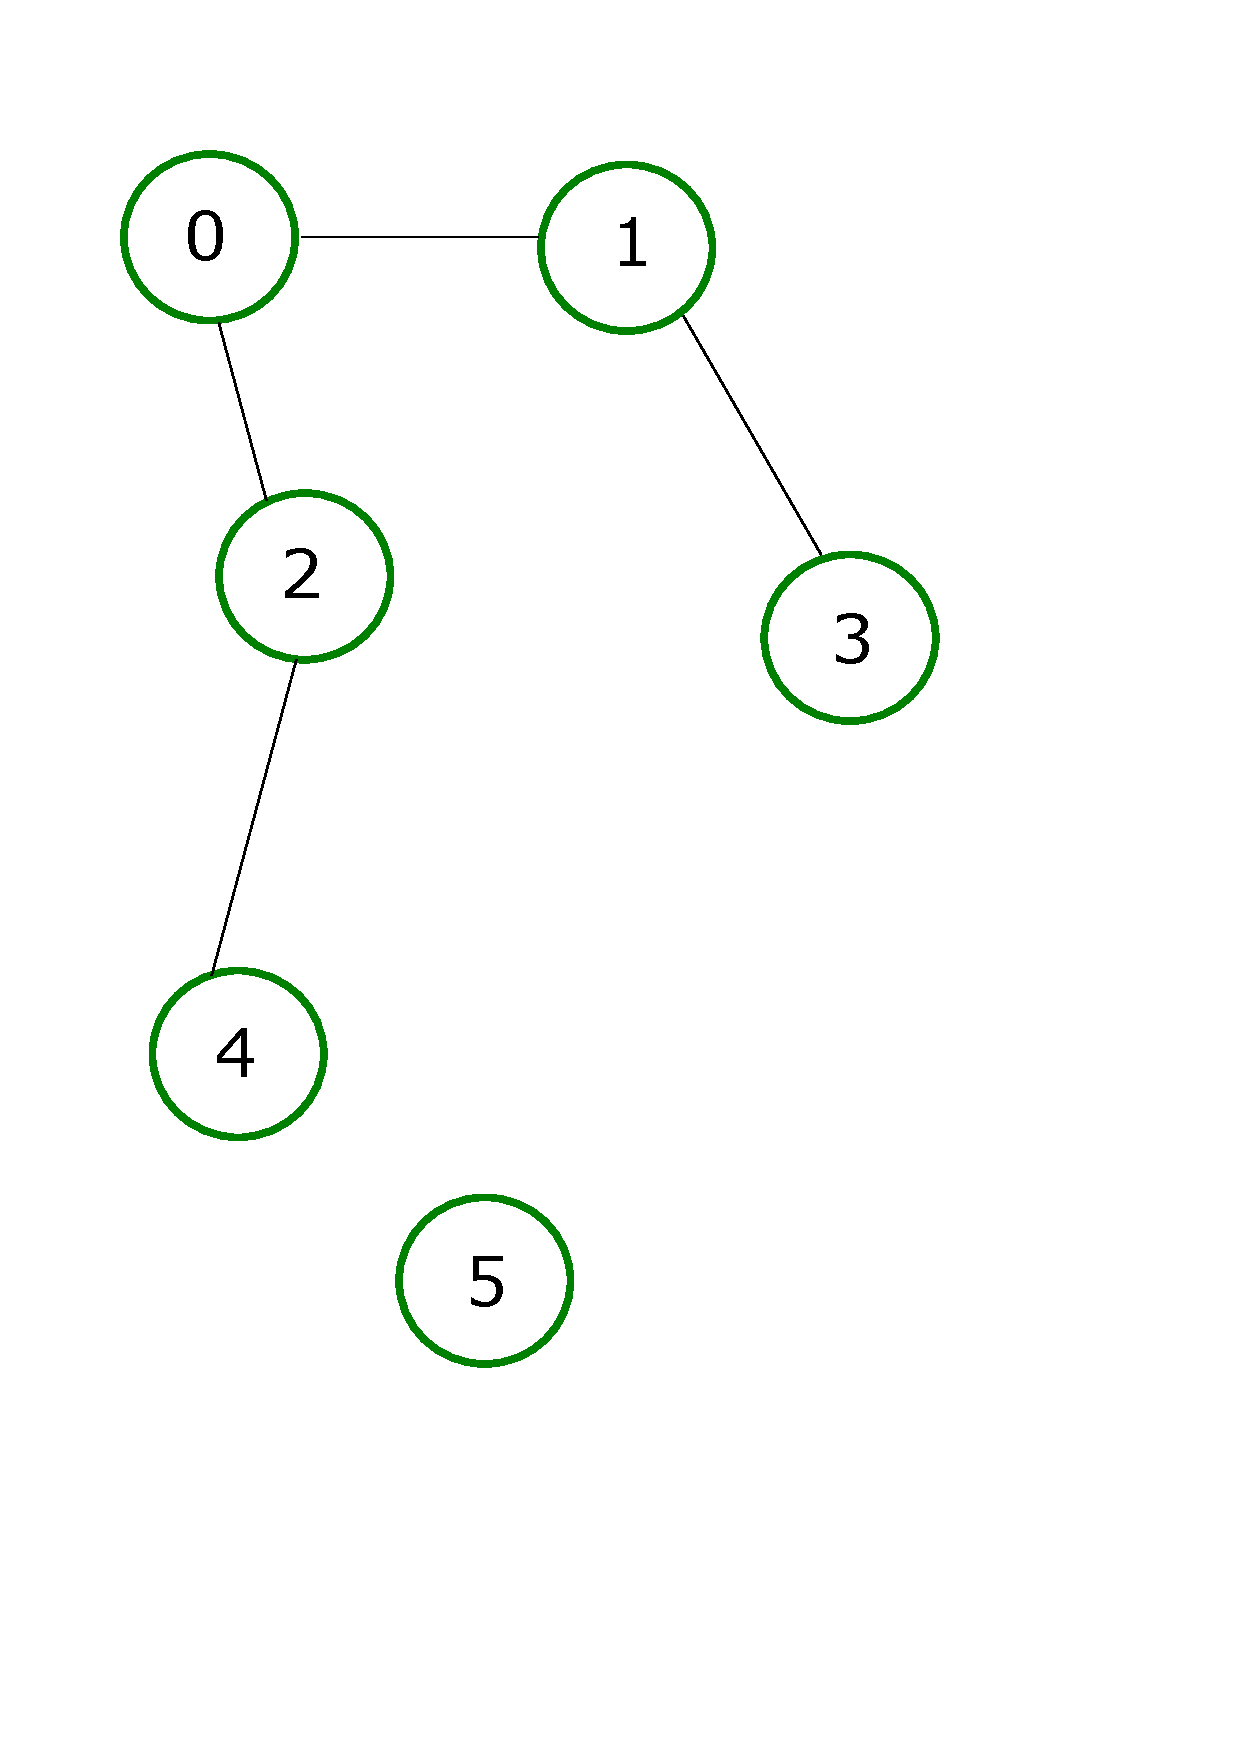
\includegraphics[scale=0.5]{nodi.pdf} 
		\caption{ASolver randomness example}
	\end{figure}
\subsection*{pros \& cons}
Pros: fast search in the node space\\
Cons: none
\section{GASolver}
\end{document}